\documentclass[xcolor=x11names,compress,professionalfonts]{beamer}

%% General packages %%%%%%%%%%%%%%%%%%%%%%%%%%%%%%%%%%
\usepackage[utf8]{inputenc}
\usepackage{graphicx}
\usepackage{tikz}
\tikzset{% change default arrow tips
    >=latex
}
\usepackage{ifthen}

\usepackage{amsmath}
\usepackage{nicefrac}

\usepackage{color}

%%%%%%%%%%%%%%%%%%%%%%%%%%%%%%%%%%%%%%%%%%%%%%%%%%%%%%


%% Beamer Layout %%%%%%%%%%%%%%%%%%%%%%%%%%%%%%%%%%
\useoutertheme[subsection=false,shadow]{miniframes}
\useinnertheme{rectangles}

\setbeamertemplate{navigation symbols}{}%remove navigation symbols

\newcommand{\btVFill}{\vskip0pt plus 1filll}%place an element at the bottom of the page

\usepackage{libertine}
\usepackage[T1]{fontenc}

\setbeamerfont{title like}{shape=\scshape}
\setbeamerfont{frametitle}{shape=\scshape}

\setbeamercolor*{lower separation line head}{bg=DeepSkyBlue4} 
\setbeamercolor*{normal text}{fg=black,bg=white} 
\setbeamercolor*{alerted text}{fg=red} 
\setbeamercolor*{example text}{fg=black} 
\setbeamercolor*{structure}{fg=black} 
 
\setbeamercolor*{palette tertiary}{fg=black,bg=black!10} 
\setbeamercolor*{palette quaternary}{fg=black,bg=black!10} 

\renewcommand{\(}{\begin{columns}}
\renewcommand{\)}{\end{columns}}
\newcommand{\<}[1]{\begin{column}{#1}}
\renewcommand{\>}{\end{column}}

\newcommand{\om}{\ensuremath{\omega}}
\newcommand{\lb}{\ensuremath{\overline{\lambda}}}
\newcommand{\zb}{\ensuremath{\overline{z}}}
\newcommand{\ham}{\ensuremath{H}}

\definecolor{BostonBlue}{HTML}{00688B}
\definecolor{Complementary}{HTML}{8B2300}
%%%%%%%%%%%%%%%%%%%%%%%%%%%%%%%%%%%%%%%%%%%%%%%%%%

\usepackage{braket}
% compile child documents using this preamble
\usepackage{subfiles}

%%%My Math

\newcommand{\pd}[2]{\frac{\displaystyle \partial #1}{\displaystyle\partial #2}} % for partial derivatives
\newcommand{\dx}{\mathrm{d}x}
\renewcommand{\d}[1]{\mathrm{d}#1}
\newcommand{\nth}{$n^\text{th}$ }

\newcommand{\mean}[1]{\langle #1 \rangle}
\DeclareMathOperator{\Pf}{Pf}
\DeclareMathOperator{\Tr}{Tr}

\begin{document}


\begin{frame}
\title{Multifractality of the tight-binding eigenstates on the Fibonacci chain}
%\subtitle{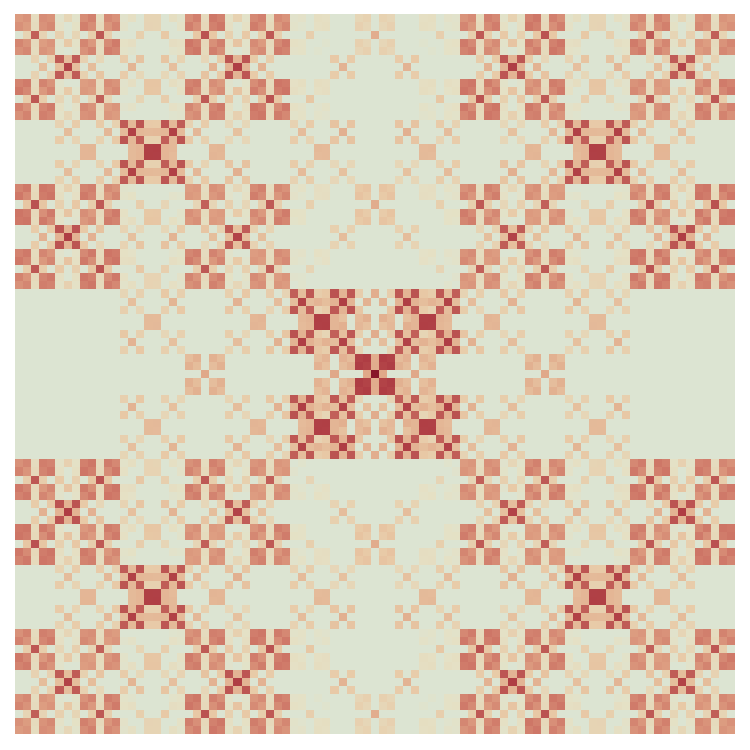
\includegraphics[width=0.2\textwidth]{illustration.pdf}}

%\titlegraphic{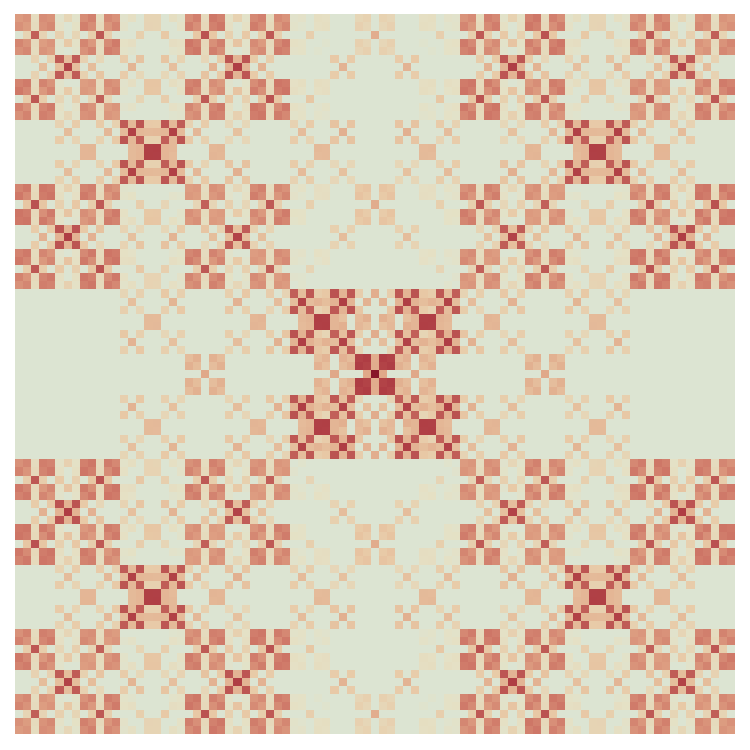
\includegraphics[width=0.4\textwidth]{illustration.pdf}}

\author{ Nicolas Macé, Anuradha Jagannathan, Frédéric Piéchon}

\institute % (optional)
{
  Laboratoire de Physique des Solides\\
  Université Paris-Sud
}

\date{September 4, 2015}

\titlepage

\btVFill
\begin{columns}
\begin{column}{2cm}
~\\
~\\
~\\
~\\
\raggedright

\includegraphics[scale=.15]{LogoUPSUD.png}
\end{column}
\begin{column}{6cm}
\centering
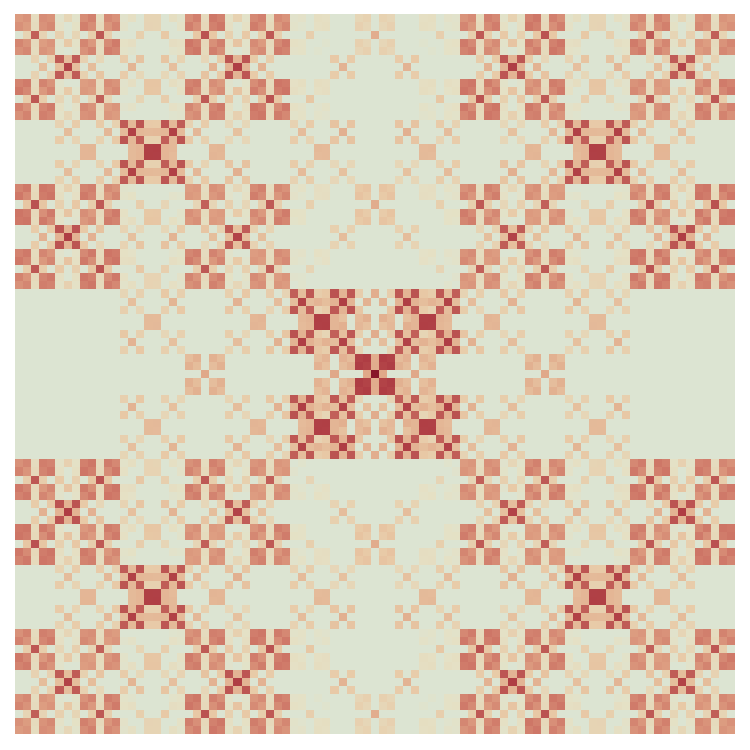
\includegraphics[width=.5\textwidth]{illustration.pdf}
\end{column}
\begin{column}{2cm}
~\\
~\\
~\\
~\\
\raggedleft

\includegraphics[scale=.15]{logo-lps.jpg}
\end{column}
\end{columns}
\end{frame}

\begin{frame}
\frametitle{Outline}
\tableofcontents[hideallsubsections]
\end{frame}

\section{The pure hopping Fibonacci Hamiltonian.}
%Each section needs a subsection for the small points on top to show up
\subsection{Dummy}

\begin{frame}{The pure hopping Fibonacci Hamiltonian}
\begin{columns}
\begin{column}{8.5cm}
	\centering
	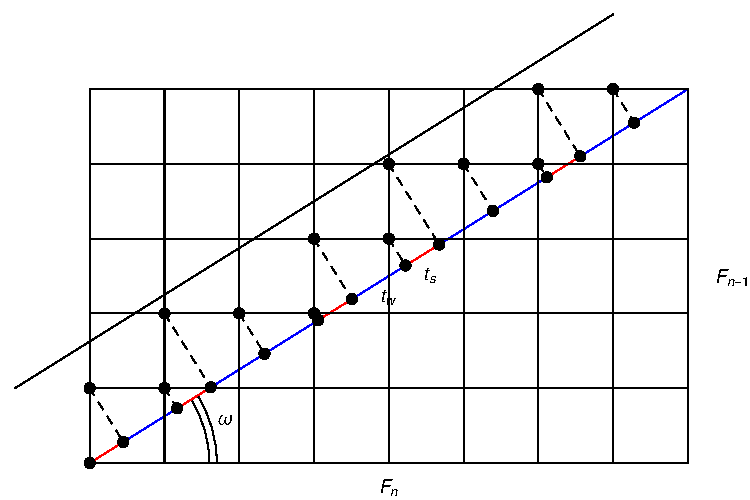
\includegraphics[scale=.65]{cut_and_project.pdf}
\end{column}

\begin{column}{3cm}
\begin{align*}
\omega_n &= \frac{F_{n-1}}{F_{n}} \\
\omega_n &\rightarrow \omega = \frac{\sqrt{5}-1}{2}
\end{align*}
\begin{align*}
\rho &= \frac{t_w}{t_s} < 1 \\
\rho &\rightarrow 1 \scriptsize{\text{ (weak modulation)}} \\
\rho &\ll 1 \scriptsize{\text{ (strong modulation)}}
\end{align*}
\end{column}
\end{columns}

	\[ \ham_n = - \sum_i t_i^{(n)} \ket{i} \bra{i+1} + \text{h.c.} \]
\end{frame}

\begin{frame}{Atoms \& molecules; decimation}
	\centering
	\begin{itemize}
	\item Atomic RG step \subfile{atomic_deflation.tex}
	\item Molecular RG step \subfile{molecular_deflation.tex}
	\end{itemize}
	\begin{flushright}
	(Niu \& Nori 1986, Kalugin, Kitaev \& Levitov 1986)
	\end{flushright}
\end{frame}

\begin{frame}{Renormalization group \& construction of the spectrum}
 \[ H_n = \underbrace{\left( z H_{n-2} - t_s \right)}_{\text{molecular sites}} \oplus \underbrace{\left( \zb H_{n-3} \right)}_{\text{atomic sites}} \oplus \underbrace{\left( z H_{n-2} + t_s \right)}_{\text{molecular sites}} + \mathcal{O}(\rho^4)\]
	$\rightarrow$ simple recursive construction of the spectrum (Niu \& Nori 1986, Piéchon \emph{et al} 1995)
	
	\begin{columns}
	\begin{column}{6cm}
	\centering
	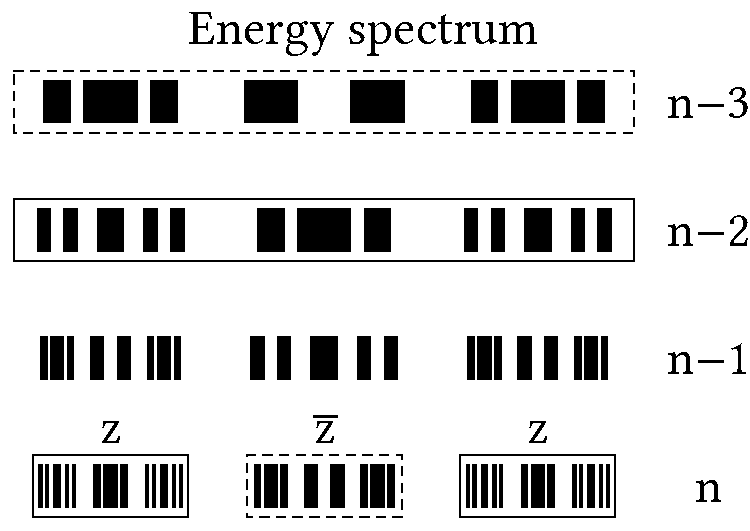
\includegraphics[scale=.45]{recursive_construction_spectrum.pdf}
	\end{column}
	\begin{column}{6cm}
	\subfile{energy_tree.tex}
	Renormalization paths characterized by
	\[ x(E) = \frac{n_+ + n_-}{n} \]
	\end{column}
	\end{columns}
\end{frame}

\section{The fractal dimensions of the spectrum.}
\begin{frame}{Fractal dimensions}
	Characterize the spectrum: multifractal analysis (Halsey \emph{et al} 1986)
	\[
	\text{Stat. properties of the bands:~} 
	\begin{cases}
	\Delta_n^a \sim (1/L_n)^{1/\alpha_a} \\
	\#\{\text{bands of scaling~} \alpha \} \sim L_n^{f(\alpha)} 
	\end{cases}
	\]
	Fractal dimensions of the spectrum: $(q-1)D_q = \min_\alpha(\alpha q - f(\alpha))$
	\begin{flushright}
	(Piéchon \emph{et al} 1995)
	\end{flushright}
	\centering
	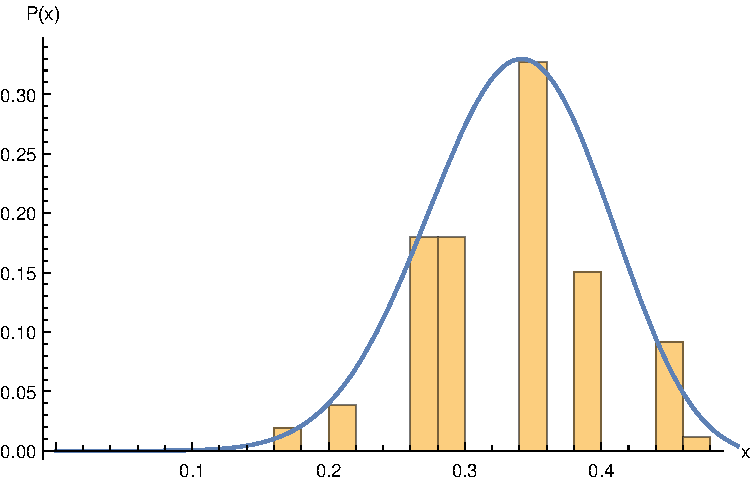
\includegraphics[scale=.45]{x_stat_th_comp.pdf}
\end{frame}

\section{The fractal dimensions of the wavefunctions.}
\begin{frame}{Fractal dimensions of the wavefunctions}
\begin{itemize}
	\item The wavefunctions are also known to be multifractal (numerical: Kohmoto?)
	\item Our work:
	\begin{itemize}
		\item Extend the perturbative RG of Niu \& Nori to describe the wavefunctions
		\item Compute the fractal dimensions of the wavefunctions
	\end{itemize}
	\item Work has already been done in this direction (Piéchon 1995, Thiem \& Schreiber 2013)
\end{itemize}
	\[
	\text{Stat. properties of $\psi$:~} 
	\int_{L_n} |\psi_n|^{2q} \sim (1/L_n)^{(q-1)D_q^\psi} 
	\]
\end{frame}

\begin{frame}{RG for the wavefunctions}
We relate the wavefunctions of $H_n$ to the wavefunctions of $H_{n-2}$, $H_{n-3}$.
\begin{itemize}
	\item We find a simple linear relation in the $\rho \ll 1$ limit: 
	\[
	\begin{cases}
		|\psi_n|^2 = \lb |\psi_{n-3}|^2 \text{~or}\\
		|\psi_n|^2 = (\lambda/2) |\psi_{n-2}|^2
	\end{cases}
	\]
	\item Similar relations for some states of the Penrose \& Amman-Beenker tight-binding Hamiltonians (Sutherland, Repetowick)
	\item When $\rho \rightarrow 1$, we obtain the exact expressions $\lambda \rightarrow \omega^2$, $\lb \rightarrow \omega^3$, well outside the validity domain of the perturbation theory.
\end{itemize}
\end{frame}

\begin{frame}{Multifractality of the wavefunctions}
\begin{itemize}
	\item Starting from the wavefunction at energy $E_n$, on the chain $n$:
		\[ |\psi_n(E_n)|^{2q} = \lambda^q \lb^q \lb^q \lambda^q ... |\psi_0(E_0)| \]
	\item The sequence $\lambda \lb \lb \lambda ...$ depends on the \emph{renormalization path} of the state $\psi$:
	\[ E_n \rightarrow E_{n-1} \rightarrow E_{n-2} \rightarrow ... \]
	\item We encode it in a number $x(\psi) \in [0,1/2)$
	\item We obtain straightforwardly the fractal dimensions:
	\[ D_q^\psi - D_q^{\psi,(0)} = - \frac{q}{q-1} \left( x(\psi) \frac{\log \lambda}{\log \omega^{-1}} + \frac{1-2x(\psi)}{3}\frac{\log \lb}{\log \omega^{-1}} \right) \]
	\[  D_q^{\psi,(0)} = x(\psi) \frac{\log 2}{\log \omega}. \]
\end{itemize}
\end{frame}

\begin{frame}{Multifractality of the wavefunctions (II)}
\begin{columns}
	\begin{column}{5cm}
		\centering
  		%\includegraphics[width=.45\textwidth]{local_wf_inset.pdf}
	\end{column}
	\begin{column}{5cm}
		\begin{itemize}
			\item States are all critical ($D_{q} < 1$ for $q > 0$)
			\item Their multifractal character is captured by our description
			\item $x$ is the master parameter in the $\rho \ll 1$ limit
		\end{itemize}
	\end{column}
\end{columns}
\end{frame}

\begin{frame}{Global multifractality}
\begin{columns}
	\begin{column}{5cm}
		\centering
		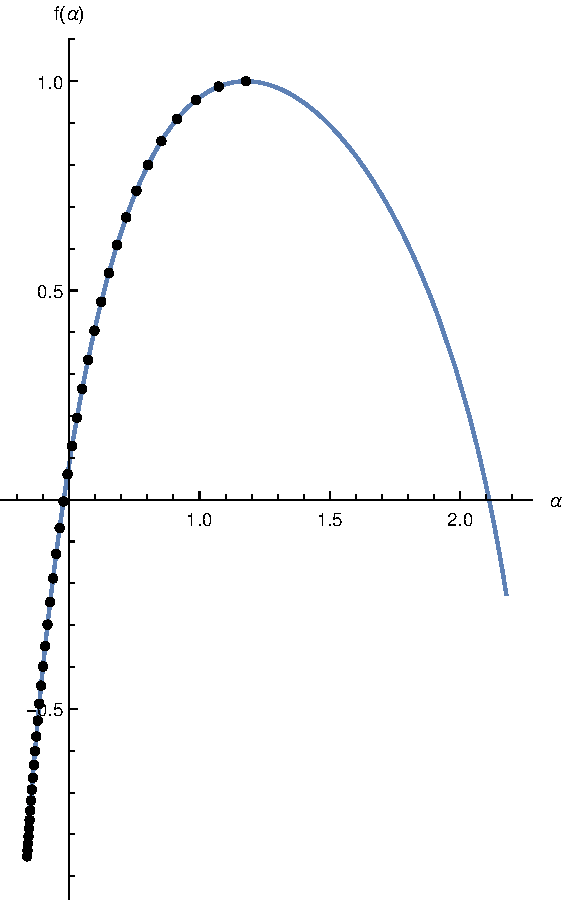
\includegraphics[scale=.5]{falpha05.pdf}
	\end{column}
	\begin{column}{5cm}
		This is the \emph{global} fractal dimensions of the wavefunctions
		\begin{itemize}
			\item Multifractality
			\item Quantitative agreement even for $\rho$ of order 1.
		\end{itemize}
	\end{column}
\end{columns}
\end{frame}

\begin{frame}{Conumbering}
\end{frame}

\begin{frame}{Conumbering in the strong quasiperiodic limit}
\end{frame}

\begin{frame}{Gap labelling \& conumberings}
\end{frame}

\end{document}
